\documentclass{article}
\usepackage{graphicx}
\usepackage{amsmath}
\usepackage{caption}

\title{Lanczos Resizing and Rotation for Image Transformation}
\author{Kunovics Dávid Zoltán}
\date{\today}

\begin{document}

\maketitle

\section{Introduction}
Image resizing and rotation are fundamental operations in image processing, commonly used in computer vision and graphics. Achieving high-quality visual results while performing these transformations simultaneously poses a significant challenge. This document describes a method implemented in MATLAB, combining Lanczos resampling for resizing and rotation using a 2D transformation matrix.

\section{Mathematical Model}

\subsection{Lanczos Resampling}
Lanczos resampling is a high-quality interpolation method based on the sinc function, defined as:
\[
\text{sinc}(x) = 
\begin{cases} 
1 & \text{if } x = 0 \\
\frac{\sin(\pi x)}{\pi x} & \text{if } x \neq 0 
\end{cases}
\]
The Lanczos kernel is constructed by multiplying two sinc functions:
\[
w(x) = \text{sinc}(x) \cdot \text{sinc}\left(\frac{x}{A}\right)
\]
where \(A\) is the kernel size parameter, controlling the range of influence of each pixel. Larger values of \(A\) yield smoother results but increase computational complexity. The kernel is truncated to \(A\) to make the computation practical:
\[
w(x) = 0 \quad \text{for } |x| \geq A
\]

\subsection{Rotation Transformation}
To rotate an image by an angle \(\theta\), we use the 2D rotation matrix:
\[
\begin{bmatrix}
x' \\
y'
\end{bmatrix}
= 
\begin{bmatrix}
\cos(\theta) & -\sin(\theta) \\
\sin(\theta) & \cos(\theta)
\end{bmatrix}
\begin{bmatrix}
x - c_x \\
y - c_y
\end{bmatrix}
+
\begin{bmatrix}
c_x \\
c_y
\end{bmatrix}
\]
where \((c_x, c_y)\) is the image center. The inverse rotation maps the rotated coordinates \((x', y')\) to the original image, enabling interpolation.

\section{Methodology}

The implementation integrates resizing and rotation in a single sampling loop using Lanczos resampling. The steps are as follows:

\begin{enumerate}
    \item \textbf{Scaling:} The target dimensions are calculated based on the scaling factor.
    \item \textbf{Inverse Mapping:} For each pixel in the output image, its coordinates are mapped back to the input image using the inverse rotation and scaling transformations.
    \item \textbf{Lanczos Interpolation:} The surrounding pixels are weighted using the Lanczos kernel, summing their contributions to compute the final pixel value.
\end{enumerate}

The kernel weights depend on the distance between the input and output coordinates, ensuring high-quality interpolation.

\section{Test Cases and Results}

The function was tested with the following configurations:
\begin{enumerate}
    \item \textbf{Test Case 1:} Rescale by a factor of 4 with no rotation (0 degrees).
    \item \textbf{Test Case 2:} Rescale by a factor of 2 and rotate by 45 degrees.
    \item \textbf{Test Case 3:} Downscale by a factor of 0.5 and rotate by 90 degrees.
\end{enumerate}

\begin{figure}[h!]
    \centering
    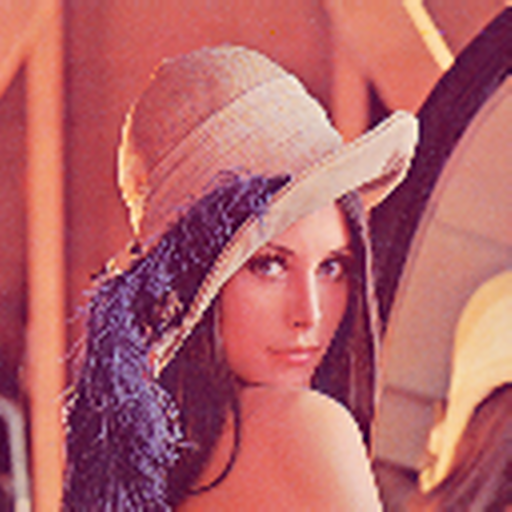
\includegraphics[width=0.4\textwidth]{lena_4.00@0.00.png}
    \caption{Test Case 1: Rescaled by a factor of 4 with no rotation.}
\end{figure}

\begin{figure}[h!]
    \centering
    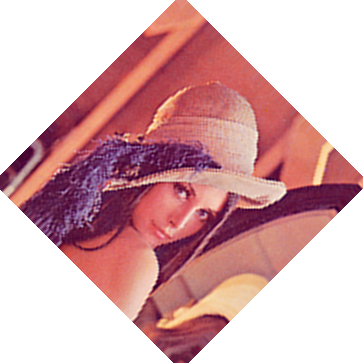
\includegraphics[width=0.4\textwidth]{lena_2.00@45.00.png}
    \caption{Test Case 2: Rescaled by a factor of 2 and rotated by 45 degrees.}
\end{figure}

\begin{figure}[h!]
    \centering
    
\includegraphics[width=0.4\textwidth]{lena_0.50@90.00.png}
    \caption{Test Case 3: Downscaled by a factor of 0.5 and rotated by 90 degrees.}
\end{figure}

\section{Conclusion}

The described MATLAB implementation demonstrates a robust approach for simultaneous resizing and rotation. By combining Lanczos resampling with inverse mapping, the method ensures high-quality transformations, preserving image details. The test cases highlight its versatility across various scales and angles.

\end{document}
